\chapter{Overview}
\label{chap:overview}
% - Overview - problem description - introduce tool - outline thesis
\section{Problem Description}

The command line is still a popular interaction medium for tooling in the areas
of software engineering and system administration. However, the usage of the
command line in the general personal computing space has practically
disappeared. This is especially true for younger individuals who from their
very first exposure to computers have been working with Graphical User
Interfaces (GUIs). This schism in interaction mediums causes issues when the
same younger individuals strive to enter technical fields such as software
development or system administration. The issue is further propagated by the
fact that because the command line is its own distinct interaction paradigm
based entirely around writing and reading text. This can mean that the usage of
traditional learning resources such as documentation and manuals might prove
difficult to translate into effective usage without active textual interaction
practice on the part of the learner. On the other hand, jumping straight into
practicing on the command line comes with its caveats. The shell can be an
unforgiving tool for a novice user as it is very sensitive to syntax and often
provides feedback that is difficult to understand for novice users. The shell
also interacts directly with the operating system and does not require
confirmation for certain destructive tasks such as file deletion.

The goal of this Master's thesis is to develop a tool that simultaneously aims
to address the previously introduced issues of lack of exposure to textual
interaction and the difficulties of traditional learning methodologies. The
tool should provide a more forgiving experience than using the shell directly
whilst still being an honest representation of shell interaction. Concepts
learned during the interactive tutorials should be directly transferrable to a
standard Unix-like shell. Furthermore, the tool should easy to use and
encourage experimentation in order to augment the learning experience and in
order to better exploit the advantages offered by interactive learning systems.


% \fig[0.75\textwidth]{img/vimtutor}{Screen shot of vimtutor}{fig:vimtutor}
\begin{figure}[htbp]
	\centering
	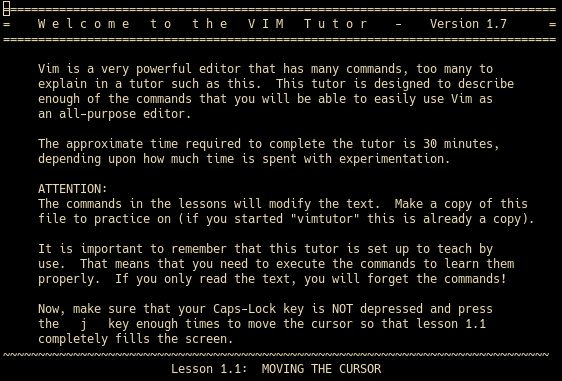
\includegraphics[width=0.75\textwidth]{img/vimtutor}
	\caption{Screen shot of vimtutor}
    \label{fig:vimtutor}
\end{figure}

\section{Introducing "CLI-Tutor"}

The \textit{CLI-Tutor} tool is an interactive shell like tutorial program for
the command line. We draw inspiration from the
`vimtutor'\cite{pierce_ware_smith_moolenaar_2019} (see: Figure
\ref{fig:vimtutor}) utility shipping alongside the popular terminal-based text
editor Vim. The \textit{CLI-Tutor} tool introduces users to topics such as
shell basics and Unix-like core utility usage through a series of interactive
examples. The tool aims to relax the steep learning curve associated with the
command line by leveraging interactive examples and a feedback mechanism to
instruct the stage of the lesson and provide some feedback based on the inputs
of the user. The core of \textit{CLI-Tutor} is contained within a command line
application written in golang\footnote{Go programming language:
\href{https://go.dev/}{https://go.dev/}} and serves as a standalone
application. However, in order to make the learning experience safer for the
user and to encourage exploration the CLI application has been wrapped into a
web application to form a sandboxed environment for the user that exposes a
terminal over the web. This means the user can use the tutorial application
without fear of causing their own system any harm. 

The \textit{CLI-Tutor} application is fully open source also comes with its own
modified parser and structure for specifying lessons based on Markdown
documents. This means that the material covered by the lessons can be easily
contributed to and distributed, making the tool quite extensible.


% \fig[0.75\textwidth]{img/clitutor}{Screen shot of CLI-Tutor}{fig:clitutor}
\begin{figure}[htbp]
	\centering
	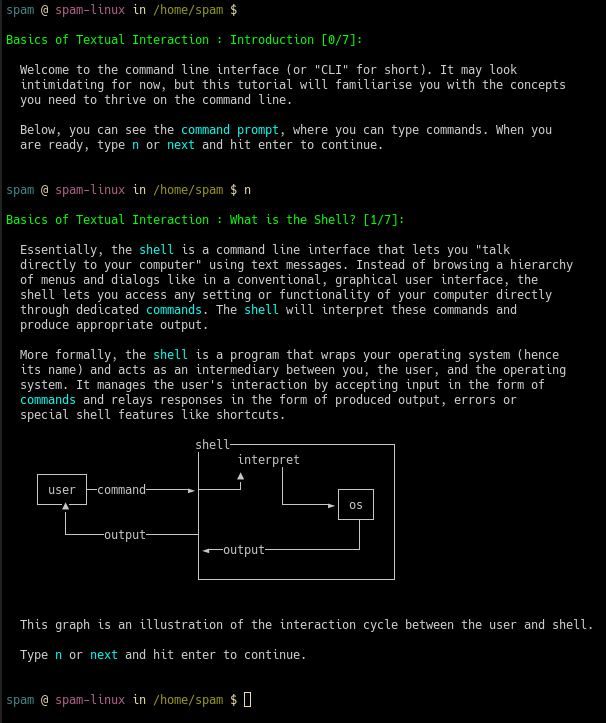
\includegraphics[width=0.75\textwidth]{img/clitutor}
	\caption{Screen shot of CLI-Tutor}
    \label{fig:clitutor}
\end{figure}

\section{Thesis Outline}

Over the next few chapters we will discuss and show the design, implementation
and overall goals of this solution. \autoref{chap:intro} will cover...

To validate the tool and answer our
research questions, a user study will be conducted, most likely with bachelor's
students at the University of Zurich. A secondary goal is to embed the learning
tool into a prototypical web application in order to make it more accessible
and portable.
This tool aims to determine whether an interactive learning method may ease the
introduction into command line interfaces for novice users, particularly
mitigating the 'scare factor' experienced by first-time users. 

\paragraph{Paragraph.} Always with a point. {}
